%\clearpage
%
%
%\section{Research Spikes}\label{sec:research-spikes}
%
%\subsection{Static (Jinja2) versus dynamic (React) webpages}\label{subsec:static-versus-dynamic-webpages}
%
%Flask allow for variables and thus data to be injected into Jinja2 Templates.
%And whenever a user tries to reach an endpoint, the server generates a HTML page based of the template filling in all the values.
%Therefore, for a large portion of static content and applications with a traditional content-driven website, this approach is sufficient for most use cases.
%
%However, when considering dynamic content, using templating becomes complex and in many cases suboptimal to other approaches.
%Javascript frameworks such as React and Angular focus on generating dynamic applications for dynamic content.
%
%A framework such as React also allows for a layer of abstraction from HTML and CSS, which allows for a quicker development cycle.
%The Javascript landscape has a huge variety of libraries and dependencies that can eliminate tedious tasks such as layout, alignment and even offers complete building blocks for pages.
%In essence, with all these tools available and also actively used in industry, developing a user interface in React reduces the tedious and low-level work, thereby providing more time for server-side development.
%
%\clearpage
%\subsection{Websocket protocol}\label{subsec:websocket-protocol}
%
%Websocket is a two-way communication protocol that allow a client to have a interactive session with the server~\cite{websocketMozilla}.
%
%\begin{figure}[H]
%    \centering
%    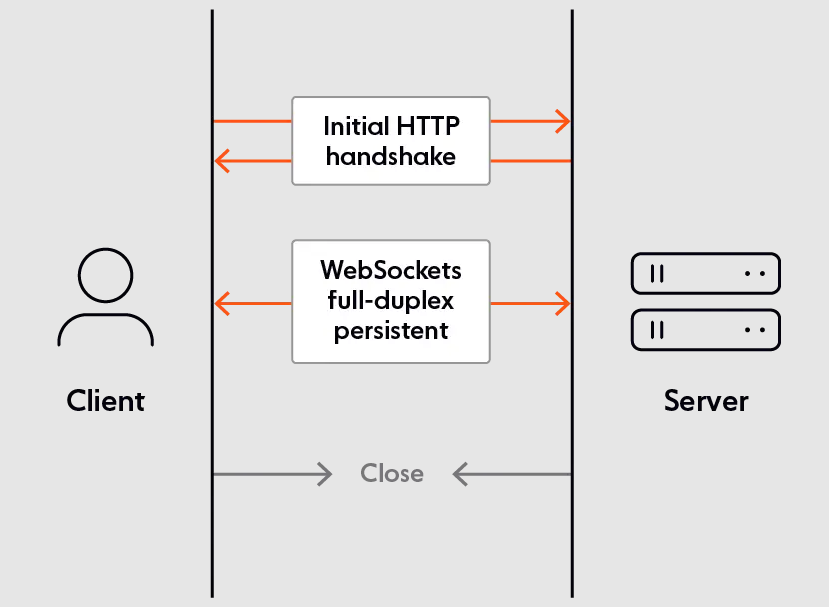
\includegraphics[width=0.5\textwidth]{../images/websockets}
%    \caption{Websocket communication \cite{diaconu}}
%    \label{fig:websocketCommunication}
%\end{figure}
%
%As shown in~\ref{fig:websocketCommunication}, the connection is established with an initial HTTP handshake.
%Once connected, the client and server can exchange data through the Websocket connection.
%The session can be closed on either side with a close message~\cite{diaconu}.
%
%\subsubsection{Why Websocket?}
%The application should be able to take many changes from many users.
%For example, if a user changes the color on square (0,0) on the grid, other users that are currently viewing the canvas should be able to receive the change without having to refresh the page.
%
%Websocket allow real-time communication and updates between the server and the client, without needing many HTTP requests.
%The protocol allow for low latency and therefore a more responsive application.
%However, Websocket unlike HTTP is a stateful protocol which introduces complexity to the server-side~\cite{diaconu}.
%
%This protocol fulfills the real-time requirement for the current use cases of the application.
%It will be an added complexity that will have to be dealt with during development, especially when considering a possible authentication system.
%
%\subsubsection{Socket.IO}
%
%Socket.IO is a library that builds on top of the WebSocket protocol that adds additional capabilities such broadcasting capabilities and compatibility concerns~\cite{socketio}.
%The library is available for both Javascript and Python Flask and can thus be used.
%
%There was a consideration for using WebSockets without Socket.IO.
%Javascript and modern browsers do have native support for the protocol through browser APIs~\cite{websocketMozilla}.
%However when looking at Flask and its implementations, the most up-to-date examples and approaches use SocketIO rather than raw WebSockets.
%This is not to say that other implementations or libraries don't exist (see \href{https://github.com/kennethreitz/flask-sockets}{flask-sockets})but SocketIO seems to be the most popular solution with an active community and developers behind it.
